\documentclass{article}
\usepackage{amssymb, amsmath, amsthm}
\usepackage[margin=1in]{geometry}
\usepackage{verbatim}
\usepackage{graphicx}
\usepackage{hyperref} % \url \href
\usepackage{docmute}

\newtheorem{definition}{Definition}
\newtheorem{theorem}{Theorem}
\newcommand{\heff}{\mathbb{H}^{\text{eff}}}
\newcommand{\pfrac}[2]{\frac{\partial #1}{\partial #2}}

\newcommand{\MO}{\textbf{MO}}
\newcommand{\AO}{\textbf{AO}}

\newcommand{\huptb}{\text{H}_0}
\newcommand{\order}[2]{#1^{(#2)}}
\newcommand{\statebra}[1]{\langle #1 |}
\newcommand{\stateket}[1]{| #1 \rangle}

\begin{document}

\section{Electronegative Perturbation}
The benefit of performing perturbation calculation is that we can first tackle 
problems with the highest symmetry possible so as to utilize symmetry to the most,
and then choose the desired approximation methods to give a more accurate 
solution. Let's first consider the case of electronegative perturbation. For simplicity, 
we consider the two orbital problem for $s$ orbitals on a diatomic molecular. This 
example also illustrates the transformation of perturbation terms from MOs to AOs. 

Let's define the unperturbed molecular to be H$_2$ molecular, whose orbital diagonal we 
have already solved. Let's write:
\begin{align*}
    \psi_1 = a (s_1 + s_2) \\ 
    \psi_2 = b (s_1 - s_2)
\end{align*}
Because of the non-neglectable overlap between the two $s$ wavefunctions, coefficients $a$ and $b$
deviate from $\sqrt{2}/2$. 
This case correspond to our high symmetry case. Suppose now one of the 
H ion is replaced by a He ion and we further suppose its only effect is to introduce:
\begin{equation*}
    \statebra{s_2} H^{(\text{He})} \stateket{s_2} = \statebra{s_2} H^{(\text{H})} \stateket{s_2} + \delta v
\end{equation*}
since He ion is more electronegative than H, $\delta V < 0$. We assume here that the interaction 
terms $\statebra{s_1} \delta H \stateket{s_2} = 0$ and orbital $\stateket{s_1}$ is also not affected. The perturbation 
can be written in matrix form:
\begin{equation*}
    \delta H^{AO} = \left(\begin{matrix}
        0 & 0 \\ 0 & \delta v
    \end{matrix}\right), \qquad 
    \delta H^{MO} = \left(\begin{matrix}
        a^2 & -ab  \\ -ab  & b^2
    \end{matrix}\right) \delta v
\end{equation*}
where the relationship $H_{ij} = \sum_{\mu \nu} c_{\mu i} c_{\nu j} H_{\mu \nu}$ is used. With this we can solve 
the perturbed molecular orbitals to first order in wavefunction and second order correction in energy:
\begin{align*}
    \psi_1' \approx \psi_1 + \frac{\tilde{H}_{12}}{\varepsilon_1 - \varepsilon_2} \psi_2 \approx \psi_1 - |t_{21}| \psi_2 \\ 
    \psi_2' \approx \psi_2 + \frac{\tilde{H}_{12}}{\varepsilon_2 - \varepsilon_1} \psi_1 \approx \psi_2 + |t_{12}| \psi_1
\end{align*}
where $\tilde{H}_{12} = -ab\cdot \delta v > 0$, and the perturbated energies to second order is:
\begin{align*}
    \varepsilon_1' = \varepsilon_1 + a^2 \cdot \delta v + \frac{(-ab\cdot \delta v)^2}{\varepsilon_1 - \varepsilon_2} \\ 
    \varepsilon_2' = \varepsilon_2 + b^2 \cdot \delta v + \frac{(-ab\cdot \delta v)^2}{\varepsilon_2 - \varepsilon_1} 
\end{align*}
We note that energy correction to first order are negative for both terms, since introducing a more electronegative ion 
lower the energies of the system in total. The sign of second order perturbation is however different.

\section{Geometry Perturbation}
When the geometry of the molecular is distorted, the perturbation in terms of molecular orbitals can found as:
\begin{align}
    \tilde{H}_{ij} &= \sum_{\mu}\sum_{\nu} c_{\mu i}^0 \delta H_{\mu \nu} c_{\nu j}^0 \\ 
    \tilde{S}_{ij} &= \sum_{\mu}\sum_{\nu} c_{\mu i}^0 \delta S_{\mu \nu} c_{\nu j}^0 
\end{align} 
If the two geometries under consideration are similar, we should have $\delta S_{\mu \nu} \to 0$. Still, the relationship
$\delta H_{\mu \nu} \propto - \delta S_{\mu \nu}$ is largely true. An non-zero geometry perturbation will change most 
of the values of matrix elements $\delta H_{\mu \nu}$ and $\delta S_{\mu \nu}$. But starting from the perturbation 
matrix $\tilde{H}_{ij}$ and $\tilde{S}_{ij}$, we can treat the geometry perturbation using the perturbation formulism 
developed. We also note that with molecualr orbitals, the diagonal overlap matrix will also be nonzero with the 
MOs are distributed on different fragments of the distorted structure. For continuous geometric perturbation, energy 
levels can be organized into \emph{Walsh diagram}, such as shown in figure \ref{F:walsh_diagram}.
\begin{figure}[h!]
    \centering
    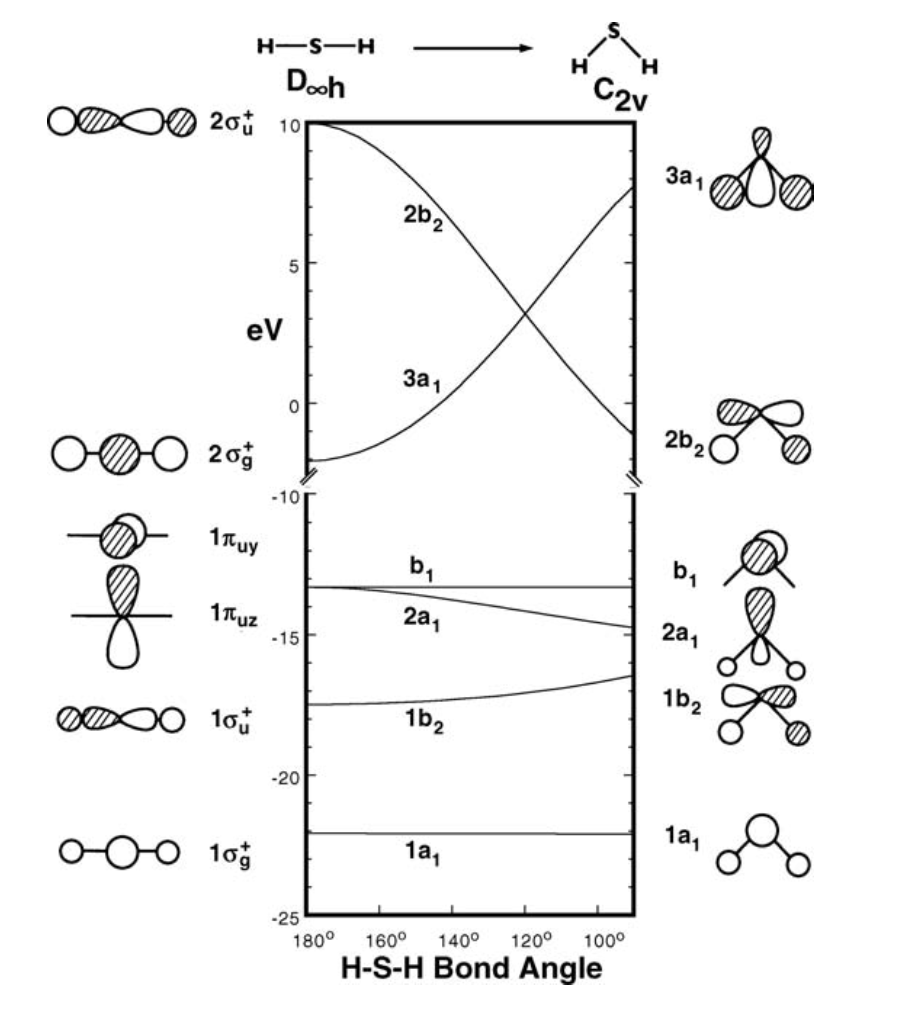
\includegraphics[width=3in]{F_walsh_diagram.png}
    \caption{Walsh diagram from a linear AH$_2$ to a trianglar AH$_2$}
    \label{F:walsh_diagram}
\end{figure}

\end{document}
